\documentclass[twoside,openright]{wfaiis}
\usepackage{polski}
\usepackage{listings}
\linespread{1.3}
\usepackage{tikz}
\usepackage{amssymb}
\usetikzlibrary{positioning}
\usetikzlibrary{snakes}
\usepackage[utf8]{inputenc}
\usepackage{graphicx}
\usepackage{url}

\autor{Łukasz Stanisławski\album{200617} }
\tytul{Symulacja ciała miękkiego z wykorzystaniem technologii CUDA}
\kierunek{informatyka stosowana}
\zaklad{Katedra Informatyki Stosowanej}
\rodzajpracy{inżynierska}
\promotor{dr hab. Jacek Matulewski}
\jednostkapromotora{Zakład Mechaniki Kwantowej}
\rok{2014}

\lstset{language=C,tabsize=2,basicstyle=\small}

\begin{document}

\maketitle

\tableofcontents

\chapter{Wstęp}

% czemu ten temat jest interesujący

% dlaczego ta praca

% co z niej można wynieść

% opis rozdziałów

\chapter{Ciało miękkie w symulacji komputerowej}

\section{Wprowadzenie}

W literaturze przedmiotu odnaleźć można szereg metod opisujących symulacje komputerowe ciał
miękkich. Metody te, mimo faktu, że potrafią symulować ten sam zakres zjawisk
fizycznych potrafią znacząco się różnić w zależności od zakresu ich zastosowań.
Symulacje fizyczne ciał miękkich będą zatem ukierunkowane na otrzymanie wyników
zbieżnych do obserwowanych doświadczalnie, natomiast te używane w grafice
komputerowej będą stawiały za cel stworzenie przyjemnego dla oka efektu
wizualnego oraz stabilność i responsywność symulacji.

Rozdział ten ma za zadanie łagodnie wprowadzić czytelnika w bogaty świat metod symulacji
ciał miękkich. Zostaną podjęte próby usystematyzowania dotychczasowych
osiągnięć w tej dziedzinie oraz pokazania w jakich obszarach stosowane są
dane typy symulacji. Rozdział ten nie ma jednak na celu dokładnego omówienia sposobów 
działania wszystkich metod, lecz tylko pobieżnym omówieniu aktualnego stanu
wiedzy a skupienie się na wybranych metodach.

Przedstawione zostaną też prawa fizyki mające zastosowanie w opisie ciał deformowalnych. Ze
względu jednak na obszerność tego zagadnienia, 
niemożliwe będzie jego wyczerpujące opisanie. Zamiast tego nacisk
zostanie położony na omówienie praw fizycznych mających zastosowanie w
konkretnych modelach opisanych w dalszej części tego rozdziału.

Spośród wielu dostępnych technik symulacji ciała miękkiego zostały wybrane
dwie najbardziej rozpowszechnione i cechujące się się
relatywnie prostą implementacją. Pomimo prostoty przedstawione w pracy
metody są podstawą współczesnych symulacji ciał
miękkich i stanowią bazę do tworzenia bardziej skomplikowanych i 
wyspecjalizowanych modeli używanych w zaawansowanych silnikach graficznych
takich jak PhysiX czy Bullet.

\section{Kategoryzacja symulacji}

Publikacje naukowe w dziedzinie symulacji ciał miękkich często mają charakter
iteracyjny. Po stworzeniu nowej metody powstają jej modyfikacje, inni badacze
poprawiają jej parametry, upraszczają,
uszczegóławiają lub nawet łączą ją z innymi znanymi technikami tworząc w ten
sposób nowe rozwiązania. W połączeniu z bardzo dynamicznym rozwojem technologii 
skutkuje to wypieraniem pewnych metod przez inne lepiej dopasowanych do obecnego
stanu wiedzy i elektroniki.

Mnogość zastosowań symulacji ciał miękkich sprawiła też, że tematyką tą
zainteresowali są badacze z różnych dziedzin. W efekcie tego obszar modelowania ciał
deformowalnych nabrał prawdziwie interdyscyplinarnego charakteru i łączy dzisiaj w sobie
taki obszary naukowe jak dynamika newtonowska, mechanika ośrodków ciągłych,
metody numeryczne, geometria różniczkowa czy metody aproksymacji\cite{pbdo}.

Bardzo zmienne środowisko, relatywnie młody wiek dziedziny czy jej 
interdyscyplinarny charakter sprawia
że obszar wiedzy na temat komputerowej symulacji ciał deformowalnych relatywnie
trudno opisać.
Jak dotąd znane są autorowi pracy tylko 2 próby usystematyzowania osiągnięć
tej dziedzinie podjęte w przeciągu ostatnich 30 lat, odnoszące się wyłącznie do
ciał miękkich.

\subsection{Metody fizyczne i niefizyczne}

Pierwszą próbę sklasyfikowania znanych metod symulacji ciał miękkich
podjęli w swoim opracowaniu z 1997 r. Sarah oraz Gibson\cite{TR97-19}. Podzielili
oni wszystkie znane modele na 2 ogólne kategorie: fizyczne oraz niefizyczne. Metody fizyczne, czyli
takie które uwzględniają w swojej budowie pewne prawa fizyczne będą przedmiotem
wnikliwszej analizy w tej pracy. Do modeli niefizycznych zaliczyć można natomiast
krzywe parametryczne oparte na krzywych Breziera czy deformacje brył sztywnych (Free-Form Deformations).\cite{pbdo}

Metody niefizyczne znajdują zastosowanie w obszarach, w których właściwości
fizyczne czy też symulacja w czasie obiektu nie ma zastosowania. Przykładem
takiego obszaru jest projektowanie komputerowe w programach typu CAD, gdzie
projektowany obiekt musi być przekształcony ze stanu A do B zachowując określone
własności. Nie dziwi zatem fakt, że wszystkie metody niefizyczne są także 
nazywane technikami geometrycznymi.

Do kategorii modeli fizycznych Sarah i Gibson zliczyli następujące klasy modeli:
\begin{itemize}
\item System Sprężyn
\item Metody ciągłe (Continuum Models)
\end{itemize}

System sprężyn będzie przedmiotem wnikliwszej analizy w dalszej części tego
rozdziału. W tym miejscu należy jednak określić zakres stosowalności tego
modelu, który obejmuje głównie grafikę komputerową oraz szeroko rozumianą
inżynierię biomedyczną. System sprężyn ze względu na swoje właściwości 
często jest wykorzystywany do symulacji tkanek ciała, gdyż pozwala łatwo łączyć ze
sobą ośrodki o potencjalnie różnych własnościach fizycznych. Dodatkowo symulacje
systemu sprężyn nie są kosztowne obliczeniowo co pozwala na stosowanie ich w
interaktywnych aplikacjach.

Drugą wymienioną w 'Survey of Deformable Modelling in Computer Graphics' jest
klasa modeli wywodząca się z teorii ośrodków ciągłych czy też mechaniki ośrodków
ciągłych. Oznacza to, że symulowany obiekt przedstawiany jest jako ciągły
fragment przestrzeni (tzw. continuum) i wykorzystuje równania różniczkowe do
opisania deformacji obiektu. Metody te znajdują zastosowanie w symulacjach
tkanek, analizie obrazów.\cite{TR97-19}

Metody bazujące na modelu continuum są bardziej fizycznie poprawne niż model
systemu sprężyn\cite{TR97-19}. Jednak posiadają one pewne niepożądane cechy.
Pierwszą jest fakt, że nie zawsze daje się znaleźć analityczne rozwiązanie
równań różniczkowych opisujących deformację ciała. Dlatego też w celu
przeprowadzenia symulacji ciała w czasie trzeba dokonać numerycznego rozwiązania
układu równań różniczkowych co wiąże się z dyskretyzacją całego modelu.

Rozwiązaniem problemu brak analitycznego rozwiązania układów równań opisujących
deformację ciała są metody pozwalające na numeryczne rozwiązanie układu. Do
metody tych zaliczamy: Metodę Elementów Skończonych (Finite Element Method),
 Metody Aproksymacyjne (Approximate Continuum Method), Metoda Róznic Skończonych
 (Method of Finite Differencies, Metoda Skończonych Objętości (Method of Finite
 Volumes). Istotną wadą modeli continuum jest ich duża złożoność obliczeniowa
czyniąca je trudnymi, lub wręcz niemożliwym do zastosowania w symulacjach czasu
rzeczywistego.

\subsection{Metody Lagrange'a i Eulera}

Drugim opracowaniem starającym się usystematyzować zagadnienia związane z
ciałami miękkimi jest 'Physically Based Deformable Models in Computer
Graphics' opublikowany w 2005 r. Według autorów sposoby modelowania ciał miękkich można
podzielić na dwie główne kategoria ze względu na sposób dyskretyzacji
obiektu w celu przeprowadzenia jego numerycznej symulacji.

\begin{itemize}
\item Metody Lagrange'a
	\begin{itemize}
	\item Metody bazujące na siatce obiektu.
		\begin{itemize}
			\item Metody ciągłe (Continuum mechanics models)
			\item System Sprężyn
		\end{itemize}
	\item Metody nie bazujące na siatce obiektu.
		\begin{itemize}
			\item Loosely Coupled Particle Systems 
			\item Smoothed Particle Hydrodynamics (SPH) 
			\item Mesh Free Methods for the solution of PDEs 
		\end{itemize}
	\end{itemize}
\item Metody Eulera
	\begin{itemize}
		\item Symulacjie płynów i gazów
	\end{itemize}
\end{itemize}

Metody Lagrange'a przedstawiają ciało miękkie jako zbiór punktów mogących
przemieszać się w czasie. Każdy punkt modelu posiada własności
charakterystyczne dla symulowanego materiału, które ewoluują wraz z ruchem
modelu\cite{pbdo}. Do definiowania ciał miękkich w metodach Lagrange'a
używane są siatki modeli, takie jak np. wykorzystywane w grafice komputerowej. 
Ze względu na użycie siatki modele Lagrange'a dzielą się na te zdefiniowane na
siatce oraz nie. Do metod zdefiniowanych na siatce zaliczamy omawiane wcześniej 
metody ciągłe oraz system sprężyn. Metody nieoparte na siatkach to przede
wszystkich systemy szeroko rozumianych cząstek.

Systemy cząstek aplikowane są głównie do symulacji rozmytych obiektów takich jak
chmury, woda, piasek, czy w ogólności do obiektów o niezdefiniowanej
powierzchni. Powstały one na potrzeby filmowych efektów specjalnych i do dzisiaj
są w tym obszarze powszechnie używane. System cząstek składa się obiektów cząstek,
reprezentowanych przez prymitywy takie jak punkt czy sfera. Każda cząstka
rozpoczyna swój cykl życia, od generacji, która łączy się z generowaniem 
jej unikalnych parametrów takich jak pozycja, prędkość, temperatura czy długość życia.
Następną fazą symulacji cząstki jest faza dynamiki, w której parametry cząstki
są aktualizowane względem czasu symulacji. Ostatecznie każda cząstka po
przekroczeniu swojej długości życie zostaje zniszczona i usunięta z modelu.
Wielką zaletą systemu cząstek jest jej nieskomplikowana budowa, co pozwala na
symulację bardzo dużych systemów cząstek. 

Drugą techniką modelowania ciał miękkich są metody Eulera. Zasadniczą różnicą
pomiędzy przytoczonymi wcześniej metodami Lagrange'a jest fakt, że nie skupiają 
się one na symulacji punktów ciała miękkiego, lecz definiują zbiór arbitralnie
określonych punktów w których wyliczane są parametry symulowanego materiału.

Typowym schematem modelowania płynów technikami Eulera jest podział przestrzeni w
której rozpatrywana jest symulacja na regularną siatkę voxeli i użycie równań Naviera-Stokes'a do
obliczenia parametrów symulacji takich jak objętość płynu w każdym voxelu,
 prędkość płynu zdefiniowana na ścianie voxela, czy ciśnienie w centrum voxela.

Metody Eulera najczęściej wykorzystywane są do symulacji płynów oraz gazów.

\section{Podstawy fizyczne}
\subsection{Prawo Hooka}
Jest jednym z pierwszych odkrytych praw fizycznych formalnie opisujących deformację ciał pod wpływam
działających na nie sił. Zostało ono odkryte w 1660 r. przez Roberta Hooka i 
stanowi bazę dzisiejszej teorii Elastyczności\cite{elast}.

Prawo Hooka jest prawem mechaniki określającym, że odkształcenie ciała jest
proporcjonalne do sił działających na ciało,
Zakładając najprostszy wariant statycznego rozciągania pręta, prawo to definiuje
się:
$$\delta = \frac{F}{S} = E\frac{\Delta l}{l}$$
$$\Delta l = \frac{lF}{SE}$$
gdzie:
F - siła działająca na pręt,
S - pole przekroju,
$\Delta l$ - wydłużenie,
$l$ - długość początkowa,
$E$ - moduł Younga

W tym miejscu zdefiniować trzeba też dwa pojęcia ważne z punktu widzenia teorii
ciał deformowalnych:
\begin{itemize}
\item naprężenie $\delta = \frac{F}{S}$ wyrażana w $Pa$,
\item odkształcenie względne $\varepsilon = \frac{\Delta l}{l}$
\end{itemize}
 
W symulacji komputerowej prawo Hooka wykorzystywane jest najczęściej do określenia sił
działających na model w wyniku jego deformacji. Takie podejście wykorzystywane
jest np. w omawianym w kolejnym podrozdziale tej pracy, modelu systemu
sprężyn, w którym to siły działająca na model próbują sprowadzić go do stanu
równowagi w którym naprężenia zgodne z w/w prawem nie występują.

\subsection{Moduł Younga}
Moduł Younga jest współczynnikiem proporcjonalności liniowej określającym
sprężystość materiałów. Określa on charakterystyczną dla danego materiału
zależność względnego między względnym odkształceniem liniowym $\varepsilon$, a
naprężeniem $\delta$.

Tak jak w fizyce, moduł Younga w symulacji komputerowej ma określać fizyczne
właściwości materiałów. Analizując literaturę przedmiotu nie znajdujemy jednak 
bezpośrednich odwołań do tej wielkości fizycznej. Zamiast tego, większość modeli wprowadza
własne bezwymiarowe wielkości mające na celu symulowanie podobnego spektrum
zachowań. I tak model systemu sprężyn wprowadza swój współczynnik
sprężystości, który jest współczynnikiem proporcjonalności między względnym
odkształceniem liniowym a działającą siłą. Modele z kategorii dynamiki
pozycyjnej, modelują właściwości materiałów poprzez wprowadzenia parametru
sztywności (stiffness) określającego tempo zbieżności danej deformacji ciała do jego
spoczynkowego stanu.

\section{Wybrane modele ciał miękkich}


\subsection{System Sprężyn}

Jedną z najczęściej wykorzystywanych technik służących do symulacji ciała miękkiego jest operowanie na siłach działających na ciało. Schemat takiej symulacji można uogólnić, zakładając, że ciało miękkie przedstawiamy jako zbiór punktów na które mogą działać siły. W każdym kroku akumulowane są siły zewnętrzne i wewnętrzne działające na każdy punkt modelu. Jako siły wewnętrzne najczęściej wymieniane są siły sprężystości czy ciśnienia, jako siły zewnętrzne siła grawitacji czy siły powstałe w następstwie kolizji z innymi obiektami. Następnie w każdym kroku symulacji z sił wyliczane jest przyspieszenie punktów zgodnie z drugim prawem dynamiki Newtona. W kolejnych krokach, wykorzystując dowolną metodę, całkujemy otrzymany układ sił obliczając prędkości, a następnie nowe pozycje punktów modelu.\cite{pbdyn}

W tym rozdziale zostanie scharakteryzowana zostanie jedna z najpowszechniejszych
fizycznych metod Lagrange'a. Jak wskazuje nazwa modelu składa się on z systemu dwóch podstawowych elementów:
\begin{itemize}
\item  Punkt Masy - punkt w przestrzeni posiadające masę, na który mogą oddziaływać siły.
\item Sprężyna - rozciągnięta pomiędzy dwoma punktami masy, posiada swoją normalną długość, nie posiada masy.

\end{itemize} 

% sześcian 2x2x2 składający się z punktów masy i sprężyn między nimi
\begin{figure}[ht]
\centering
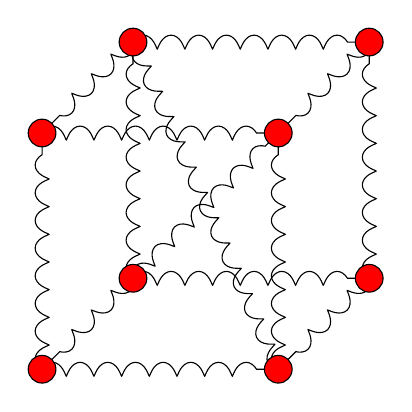
\begin{tikzpicture}

    \draw[-,snake=coil] (0,0 ,0) -- (0,3 ,0);
    \draw[-,snake=coil] (0,0 ,3) -- (0,3 ,3);
	\draw[-,snake=coil] (3,0 ,0) -- (3,3 ,0);
	\draw[-,snake=coil] (3,0 ,3) -- (3,3 ,3);
	\draw[-,snake=coil] (0,0 ,0) -- (3,3 ,3);
	\draw[-,snake=coil] (3,0 ,3) -- (0,3 ,0);
\foreach \y in{0,3}
{
    \draw[-,snake=coil] (0,\y ,0) -- (3,\y ,0);
    \draw[-,snake=coil] (0,\y ,3) -- (3,\y ,3);
	\draw[-,snake=coil] (0,\y ,0) -- (0,\y ,3);
	\draw[-,snake=coil] (3,\y ,0) -- (3,\y ,3);

	\filldraw[fill=red, draw=black] (0, \y, 0) circle (5pt);
	\filldraw[fill=red, draw=black] (3, \y, 0) circle (5pt);
	\filldraw[fill=red, draw=black] (0, \y, 3) circle (5pt);
    \filldraw[fill=red, draw=black] (3, \y, 3) circle (5pt);
}

\end{tikzpicture}

\caption{Zbiór punktów masy z przykładowym układem połączeń}
\end{figure}

%
% Równanie ogólne siły działającej na punkt masy
%
\begin{equation}
F_{i} = \sum_{j} g_{ij} + f^{d}_i + f^{ex}_{i}
\end{equation}

W powyższym równaniu na punkt masy w danej chwili $t$ działają siły:
\begin{itemize}
\item  Sprężystości $g_{ji}$ generowane przez sprężyny zawieszone między sąsiadującymi punktami.

\begin{equation}
g_{ij} = k_s (| x_{ij}| - l_{ij})\frac{x_{ij}}{|x_{ij}|}
\end{equation}
,gdzie $x_{ij} = x_i - x_j$, jest wektorem różnicy położeń między sąsiadującymi punktami masy. Siła sprężystości w modelu jest zgodna z prawem Hook'a, czyli jest proporcjonalna do odchylenia sprężyny od jej spoczynkowej długości $l_{ij}$. Współczynnik $k_s$ jest współczynnikiem sprężystości i z założenia jest zależny od materiału z którego składa się symulowane ciało.

\item Tłumienia $f^{d}_i$ wynikająca z faktu, iż symulowanie ciało nie jest doskonale elastyczne i nie zachowuje energii układu. (Tzn. energia mechaniczna jest transformowana w energię wewnętrzną ciała, jednak z punktu widzenia symulacji energia nie jest zachowana.)

\begin{equation}
f^{d}_i = k_d(v_j - v_i)
\end{equation}
,gdzie $v_i$ i $v_j$ są wektorami prędkości dwóch punktów masy połączony sprężynami, a $ k_d$ jest współczynnikiem tłumienia charakterystycznym dla symulowanego materiału.

\item Zewnętrzne $f^{ex}_{i}$ działające na punkt materialny, takie jak np. grawitacja.
\end{itemize}. 

Zdefiniowany model jest w istocie równaniem różniczkowym drugiego rzędu i może
być rozwiązany jednym z wielu algorytmów numerycznych. Jedną z najczęściej
wykorzystywanych metod jest algorytm Verleta, który cechuje się prostotą, dając
jednocześnie wystarczająco dokładne rozwiązania. Badania przeprowadzone w \cite{var} pokazały, że algorytm Verleta okazał się najwydajniejszy w porównaniu z innymi metodami numerycznymi, dlatego też będzie stosowany w niniejszej pracy.

Wzór na pozycję punku masy w czasie $t + dt$ jest w modelu wyrażona wzorem:

% Wzór na dynamikę punktu w modelu (Verlet)
\begin{equation}
x_i(t + dt) = \frac{F_i(t)}{m} dt^2 + 2x_i(t) - x_i(t - dt)
\end{equation}

Ze względu na fakt, iż niektóre siły są zależne od poprzednich prędkości punktu masy, do symulacji wykorzystywane będzie też wariant prędkościowy algorytmu Verleta. Jest on zapisany wzorem:

% Wzór na dynamikę punktu w modelu (prędkościowy Verlet)
\begin{eqnarray}
x_i(t + dt) = \frac{F_i(t)}{2m} dt^2 + x_i(t) + v_i(t)dt \\
v_i(t + dt) = \frac{F_i(t + dt) + F_i(t)}{2m}dt + v_i(t)
\end{eqnarray}

%
% MODYFIKACJE MODELU
%
\subsubsection{Modyfikacje modelu}

\subsubsection{Siła tłumienia}
Siła tłumienia zdefiniowana jako różnica prędkości między dwoma punktami masy w podstawowym modelu jest rzadko stosowana, ze względu na wiele niepożądanych własności. Tłumi ona np. obrót ciała wokół nieruchomego punktu masy, jak przedstawiono na rys. \ref{tlumienie}.

\begin{figure}[ht]
\centering
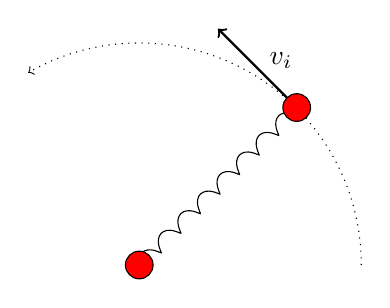
\begin{tikzpicture}

\draw[->,dotted,] (2.82,0) arc (0:120:2.82) ;
\draw[-,snake=coil] (0,0) -- (2,2);
\draw[->, thick] (2,2) -- (1,3);
\filldraw[fill=red, draw=black] (0,0) circle (5pt);
\filldraw[fill=red, draw=black] (2,2) circle (5pt);
\draw (1.8, 2.6) node {$v_i$};
\end{tikzpicture}


\caption{Rotacja wokół nieruchomego punktu}
\label{tlumienie}
\end{figure}

Według \cite{pbdo} przyjęcie prostej różnicy prędkości punktów w przypadku symulacji materiałów tłumi ich pożądane własności, takie jak podatność na gięcie i marszczenie. Dlatego też warunek na siłę tłumienia zdefiniujemy jako:
\begin{equation}
f^{d}_i = k_d (\frac{v_{ij}^\intercal x_{ij}}{x_{ij}^\intercal x_{ij}}) x_{ij}
\end{equation}

,gdzie $v_{ij} = v_i - v_j$. Powyższe równanie wyznacza siłę tłumienia modelu równą iloczynowi współczynnika tłumienia i projekcji różnicy prędkości dwóch punktów masy na wektor ich różnicy położeń. Definicja nakłada zatem ograniczenie, iż siła tłumienia może działać tylko w tym samymi kierunku co wektor różnicy położeń.

\subsubsection{Zachowanie objętości}
Kolejnym, istotnym aspektem symulacji ciała miękkiego jest zachowanie jego
objętości. System punktów mas i sprężyn nie symuluje obiektów posiadających
objętość, także często może się zdarzyć, że układ znajdzie się w stanie
stabilnym, jednak różnym od wyjściowego. W praktyce często oznacza to, że w
wyniku działania dużych sił elementy modelu zostaną obrócone lub zapadną się w
swoją własną strukturę. Przykład tego jest przedstawiony na rysunku \ref{stany}.

\begin{figure}[ht]
\centering
\includegraphics[width=7cm, height=7cm]{images/stabilny.png}
\includegraphics[width=7cm, height=7cm]{images/niestabilny.png}
\caption{Dwa stany stabilne dla sześciennego modelu.}
\label{stany}
\end{figure}

Rozwiązaniem problemu przechodzenia układu między stanami stabilnymi okazało się wprowadzenie sztucznej siły, pozwalającej zachować objętość. Takie podejście po raz pierwszy zaproponowano w \cite{rmofa}. Autorzy publikacji pogrupowali znajdujące się w układzie punkty masy w obiekty dla których można było zdefiniować objętość. Następnie w zależności od różnicy pomiędzy objętością spoczynkową a aktualną generowana była siła oddziałująca punkty masy. Kierunek tej siły jest zgodny z działaniem pewnej z góry zdefiniowanej normalnej. W \cite{isodb} autorzy przedstawiają bardziej ogólny przypadek przyjmując, że obiektem posiadającym objętość jest czworościan.Wierzchołki figury są punktami masy, a krawędzie sprężynami. Siła zachowawcza działająca na dany punktu masy $i$ czworościanu, określa się wzorem:

\begin{equation}
F_i^d = d_v ( v - v_0) n_i
\end{equation}
,gdzie $v$ jest aktualną objętością symulowanego czworościanu, $v_0$ jest jego spoczynkową objętością a $d_v$ jest arbitralnie zdefiniowaną stałą. $n_i$ jest to normalna przeciwległej ściany czworościanu. Podana metoda pozwala uniknąć odwrócenia wierzchołków symulowanego obiektu, ponieważ w takim przypadku obliczona objętość będzie ujemna i powstała, duża siła $F_i^d$ wymusi powrót układu do stanu wejściowego \cite{isodb}.

\subsubsection{Zależność od topologii}
W analizowanym modelu topologia połączeń między punktami mas jest z góry zdefiniowana. Można powiedzieć, że jest to kolejny parametrem symulacji, który w istotny sposób decyduje o jej jakości. Takie założenie samo w sobie nie jest błędne, gdyż modelując wewnętrzną strukturę ciała możemy określić jego fizyczną charakterystykę. Na przykład, symulując elastyczny sześcian i dodając dodatkowe połączenia między punktami masy w jednej płaszczyźnie otrzymamy obiekt różnie podatny na odkształcanie w zależności od kierunku działania siły. Taką mechaniczną właściwość ciała nazywany anizotropią. Anizotropia stanowi bardzo ciekawy przykład własności mechanicznej materiału, której implementacji w modelu punktów mas i sprężyn jest często problematyczna. 

Idealny model powinien umożliwiać symulowanie materiałów izotropowych (o własnościach mechanicznych niezależnych od kierunki działań siły) jak i anizotropowych. Poprzez możliwość manipulacji rozmieszczeniem punktów materialnych, sposoby ich połączeń sprężynami czy manipulowanie stałymi sprężystości, model dostarcza narzędzi do implementacji tych własności. Nie mniej jednak niektóre własności mogą pojawiać się wbrew wcześniejszym założeniom. Przykład niepożądanej anizotropii, otrzymanej poprzez różne struktury wewnętrzne modelu przedstawiono na rys. \ref{anizotropia}.

\begin{figure}[ht]
\centering
\includegraphics[scale=0.5]{images/anisotropy.png}
\caption{Porównanie dwóch zastosowanych siatek w obiekcie przytwierdzonym górną podstawą i poddanemu sile grawitacji. Lewo: Anizotropia obserwowana w czworościennej siatce połączeń. Prawo: Brak anizotropii w sześciennej siatce połączeń. Źródło: \cite{ca}}
\label{anizotropia}
\end{figure}

Okazuje się, że kalibracja parametrów modelu nie jest trywialna. W \cite{usa} autorzy proponuję metodę kalibracji poszczególnych stałych sprężystości sprężyn. Ich metoda pozwala na symulację zarówno izotropowych jak i anizotropowych. Jednak jak sami autorzy wskazują jest złożona obliczeniowo,a w publikacji została zaprezentowany tylko przykład dla siatek dwuwymiarowych. Inne podejście w swojej publikacji przedstawili francuscy badacze wykorzystując do estymacji parametrów sprężystości algorytmy genetyczne.\cite{ei}

Alternatywne podejście, odchodzące nieco od klasycznego modelu punktów mas i sprężyn, zostało przedstawione w publikacji D. Bourguignon i M-P. Cani \cite{ca}. Metoda ta, pochodna od systemu punktów mas i sprężyn, pozwala na definiowanie własności mechanicznych symulowanych obiektów niezależnie od przyjętej geometrii czy topologii. Pozwala to na wczytanie do symulacji obiektów utworzonych w programach do modelowania 3D i co ważniejsze, odciążenia grafika z konieczności uwzględnienia podczas pracy fizycznych charakterystyk modelu.\cite{ca}

Metoda zakłada, wszystkie punkty masy w modelu są pogrupowane w tzw. jednostki objętości (volume element), którymi najczęściej są czworościany. Dla każdej jednostki wyznacza się tymczasowe punkty masy położone wzdłuż stałych, predefiniowanych osi. Umiejscowienie osi ma odzwierciedlać mechaniczną charakterystykę obiektu. Z reguły stosuje się standardowo 3 osie, jednak możliwa jest też ich większa ilość \cite{ca}. Sposób wyznaczania punktów przecięcia przedstawiony jest na rysunku \ref{anizotropia-czworoscian}.

\begin{figure}[ht]
\centering
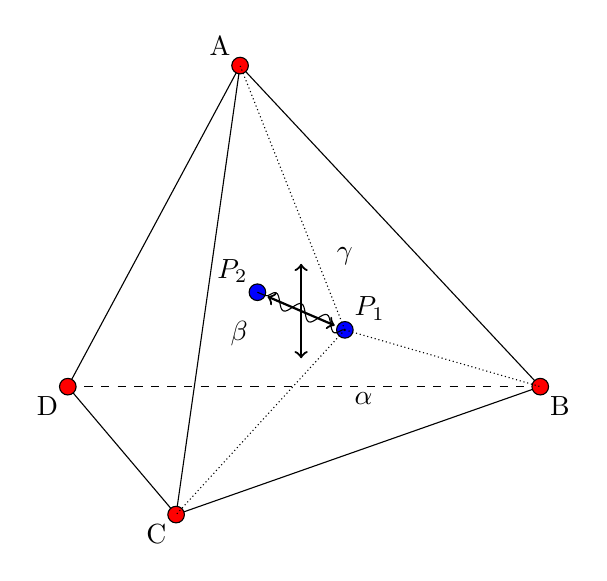
\begin{tikzpicture}

\coordinate (A) at (0, 0, 0);
\coordinate (B) at (6, 0, 0);
\coordinate (C) at (3, 0, 4.22);
\coordinate (D) at (3, 4.89, 2.11);

\draw[-] (D) -- (B) -- (C) -- (D) -- (A) -- (C);
\draw[-, dashed] (A) -- (B);

\filldraw[fill=red, draw=black] (A) circle (3pt);
\filldraw[fill=red, draw=black] (B) circle (3pt);
\filldraw[fill=red, draw=black] (C) circle (3pt);
\filldraw[fill=red, draw=black] (D) circle (3pt);

\node[above left] at (D) {A};
\node[below right] at (B) {B};
\node[below left] at (C) {C};
\node[below left] at (A) {D};

%intersection points
\coordinate (I1) at (barycentric cs:D=0.5,B=0.7,C=0.5);
\coordinate (I2) at (barycentric cs:A=0.7,B=0.5,D=0.5);
\coordinate (Imid) at (barycentric cs:I1=0.5,I2=0.5);

\filldraw[fill=blue, draw=black] (I1) circle (3pt);
\filldraw[fill=blue, draw=black] (I2) circle (3pt);
\node[above right] at (I1) {$P_1$};
\node[above left] at (I2) {$P_2$};
\node[below=25pt, right] at (I1) {$\alpha$};
\node[below=15pt, left] at (I2) {$\beta$};
\node[right, above=20pt] at (I1) {$\gamma$};

\draw[-,snake=snake] (I1) -- (I2);
\draw[<->,thick, shorten >=4pt, shorten <=4pt] (I1) -- (I2);
\draw[->,thick] (Imid) -- ++(0,0.6,0);
\draw[->,thick] (Imid) -- ++(0,-0.6,0);

\draw[-,densely dotted] (I1) -- (C);
\draw[-,densely dotted] (I1) -- (D);
\draw[-,densely dotted] (I1) -- (B);


\end{tikzpicture}

\caption{Wyznaczanie punktu przecięcia z osiami w czworościanie.}
\label{anizotropia-czworoscian}
\end{figure}

Przedstawiony czworościan posiada zdefiniowane dwie osie. Wyznaczono też dwa punkty przecięcia $P_1$ oraz $P_2$ z osią poziomą figury. W celu zapamiętania pozycji punktów przecięcia wyznacza się współczynniki kombinacji liniowej z wierzchołkami tworzącymi ścianę. $P_1 = \alpha * A + \beta *B + \gamma *C$. Współczynniki te muszą być wyznaczane dla czworościanu znajdującego się w stanie spoczynku. Punkty przecięcia traktowane są odtąd jak nowe punkty masy. Działają na nie siły wewnętrzne i zewnętrzne układu. Dwa punkty (zaznaczonymi na rys. \ref{anizotropia-czworoscian} kolorem niebieskim) zostają w istocie połączone sprężyną.

Następnie dokonuje się omawianych w poprzednich podrozdziałach obliczeń sił działających na punkt przecięcia. Mając dane współczynniki kombinacji liniowej, wyznaczyć można siły działające na punkty masy $A,B,C$ pierwotnie zdefiniowane w modelu. 

\begin{figure}[ht]
\centering
\includegraphics[scale=0.5]{images/fixed_anisotropy.png}
\caption{Porównanie dwóch zastosowanych siatek w obiekcie przytwierdzonym górną podstawą i poddanemu sile grawitacji. W modelu wykorzystano metodę D. Bourguignon i M-P. Cani, Źródło: \cite{ca}}
\label{anizotropia-czworoscian-fix}
\end{figure}

\subsection{Metody bazujące na pozycji}
Metody bazujące na pozycji są relatywnie młodą metodą wykorzystywaną w symulacji
ciał miękkich. Pierwsze propozycje takiego podejścia przedstawione zostało w
roku 2001 r.\cite{jak}, natomiast uogólniona wersja będąca bazą kolejnych
iteracji modelu, została oficjalnie opublikowana w 2006 r.\cite{pbdyn}. Metody te
szybko stały się popularne w obszarze grafiki komputerowej i jest dzisiaj
implementowana w profesjonalnych silnikach fizycznych takich jak PhysiX czy
Bullet.

Model przedstawiony w tej pracy jest fizycznym modelem Lagrange'a. Termin
bazujący na pozycji oznacza, że w odróżnieniu od symulacji bazujących na siłach, to pozycje
wszystkich punktów materialnych symulowanego ciała podlegają w symulacji pewnym
regułom. Zastosowania reguł, czy jak to będzie zwane później ograniczeń, na
punkty modelu skutkuje poprawą stabilności symulacji oraz ułatwia jej
implementację. Do najważniejszych zalet modeli bazujących na pozycji należą:
\begin{itemize}
	\item bezpośrednia kontrola nad całkowaniem równań ruchu, pozwala rozwiązań
	problemy z niestabilnością model.
	\item punkty materialne mogą być bezpośrednio manipulowane, bez użycia sił.
	\item model ograniczeń bazujących na pozycji może być wykorzystany do
	symulowania szerokiego zakresu zdarzeń fizycznych.
	\item system rozwiązujący ograniczenia w modelu jest łatwy w implementacji.
\end{itemize}

\subsubsection{Definicja}
Model zakłada, że każdy obiekt deformowalny jest przedstawiony jako zbiór $N$
punktów materialnych (zwanych dalej wierzchołkami) oraz $M$ ograniczeń
zdefiniowanych na tych wierzchołkach. Każdy i-ty wierzchołek modelu posiada
następujące atrybuty:

\centering
\begin{tabular}{|r|l|}
\hline
$x_i$ & pozycja w $R^3$ \\
\hline
$v_i$ & prędkość \\
\hline
$m_i$ & masa\\
\hline
\end{tabular}

\raggedright
Natomiast j-te ograniczenie posiada następujące atrybuty:

\centering
\begin{tabular}{|r|l|}
\hline
$n_j$ & liczność ograniczenia \\
\hline
$C_j$ & funkcja $R^{3n_j} -> R$\\
\hline
${i_1, ..., i_{n_j}}, i_k \in [1,..N]$ & zbiór indeksów\\
\hline
$k_j \in [0.. 1]$ & sztywność\\
\hline
typ & równość lub nierówność\\
\hline
\end{tabular}

\raggedright
Dane j-te ograniczenie typu równości jest spełnione wtedy gdy $C_j(x_{i_1},...,
		x_{i_{n_j}}) = 0$, natomiast typu nierówności wtedy gdy $C_j(x_{i_1},...,
		x_{i_{n_j}}) > 0$. Parametr $k_j$ definiuje siłę ograniczenia w
		przedziale od $0...1$, gdzie 0 oznacza ograniczenie, które nie powoduje
		przemieszczenia symulowanych wierzchołków, natomiast 1 oznacza, że
		wierzchołki muszę tak zostać przesunięte aby spełnić ograniczenie w
		danym kroku symulacji.

\paragraph{Algorytm}

Mając dany model $\{X_N, C_M, \Delta t \} $ każda iteracja symulacji przebiega
następująco:
\begin{enumerate}
\item \textbf{for} $i = 1:N$
\item \hspace{1cm} $x_i = x_i^0, v_i = v_i^0, w_i = 1/m_i$
\item \textbf{end for}
\item \textbf{loop}
\item \hspace{1cm} \textbf{for} $i = 1:N$ \textbf{do} $v_i \leftarrow v_i + \Delta t w_i f_{ext}(x_i)$
\item \hspace{1cm} \textbf{for} $i = 1:N$ \textbf{do} $p_i \leftarrow x_i + \Delta t v_i$
\item \hspace{1cm} \textbf{for} $j = 1:liczbaIteracjiSolwera$
\item \hspace{2cm} $rozwiazOgrnaiczenia(C_1,..., C_{M}, p_1, ..., p_N)$
\item \hspace{1cm} \textbf{end for}
\item \hspace{1cm} \textbf{for} $i = 1:N$
\item \hspace{2cm} $v_i = (p_i - x_i) / \Delta t$
\item \hspace{2cm} $x_i = p_i$
\item \hspace{1cm}\textbf{end for}
\item \textbf{end loop}

\end{enumerate}

W zaproponowanej przez Mullera symulacji bazującej na pozycji, najważniejszą częścią stanowią są
fragmenty (6), (8), (11-12). W linii (6) następuje całkowanie równania ruchu za 
pomocą metody Eulera, ustala się w ten sposób predykcję pozycji $p_i$. Następnie
wszystkie predykcje są rzutowane w taki sposób aby spełniły wszystkie
ograniczenia $C_M$. Ostatnim krokiem symulacji jest ponowne wyliczenie
prędkości oraz przypisane zrzutowanej predykcji do pozycji wierzchołka.

Model pozwala do włączenia do symulacji sił zewnętrznych $f_{ext}$, którymi na ogół jest
grawitacja. W celu symulowania innych sił działających na symulowane ciało
operuje się bezpośrednio na prędkościach wierzchołków, które mogę zostać
zmienione pomiędzy liczeniem predykcji, (między 5-6) oraz po
zaktualizowaniu pozycji oraz prędkości (13-14).

Przedstawiona symulacja jest bezwarunkowo stabilna ponieważ nowe pozycje nie są
ekstrapolacją wynikająca z kroku całkowania (6), tyko pewnym rzutowaniem na
stabilne konfiguracje systemu wyliczane podczas iteracji solwera (8). Jedynym
źródłem niestabilności jest sam solwer, którym używa metody Newtona do wyliczenia
stabilnej konfiguracji. Jednakże niestabilność nie zależy od przyjętego kroku
całkowania systemu $\Delta t$, tylko od samej funkcji danego
ograniczenia\cite{pbdyn}.

\subsubsection{Rozwiązywanie układu ograniczeń}
Problem rozwiązania ograniczeń $C_1, .., C_M$ dla projekcji układu $p_1, ..., p_N$
jest podobny do problemu rozwiązania układu równań. Do rozwiązania takiego
układu możemy się posłużyć metodami Jacobiego oraz Gaussa-Seidela. 

Niestety, w modelu funkcje ograniczeń mają też postać nierówności, a
najczęściej spotykane funkcje ograniczeń mają charakter nieliniowy. Powoduje to,
że niemożliwe jest użycie klasycznych wersji w/w metod. Muller proponuje
zmodyfikowana metodę, w której to każde równanie (lub nierówność) będzie rozwiązane
oddzielnie metodą Newtona, a następnie otrzymane rozwiązanie zostanie użyte w
następnej iteracji solwera. Zmodyfikowana metoda Gaussa-Seidela dodatkowo używa
poprzedniego rozwiązania równania do estymacji następnego co skutkuje szybszą
zbieżnością metody\cite{pbdyn}.

\subsubsection{Ograniczenia}
Ograniczenia mają za cel rzutowanie wyliczonej projekcji $p_i$ do przestrzeni
rozwiązań możliwych. Spełnienie warunków ograniczenia oznacza w 
modelu pozycyjnym przemieszczenie danej projekcji wierzchołka o wektor $\Delta p$.
Jeżeli dane ograniczenie modeluje zależności między punktami należącymi do
obiektu to przesunięcie $\Delta p$ powinno posiadać
pewne pożądane z punktu widzenia symulacji własności: zachowanie pędu oraz
momentu pędu.

Pęd jest zachowane jeśli przesunięcie $\Delta p$ posiada własność:
$$ \sum_i m_i \Delta p_i = 0$$
Natomiast moment pędu jest zachowany gdy:
$$ \sum_i r_i \times m_i p_i = 0$$, gdzie $r_i$ jest odległością $p_i$ do punktu
rotacji.

Nie spełnienie w/w równości skutkuje powstawaniem dodatkowych sił, które
oddziałują na punkty obiektu tak jak siły zewnętrzne. Jeżeli dane ograniczenie
nie dotyczy zewnętrznych właściwości (np. odległości od punktu kolizji),
własności te nie muszą być zachowane\cite{pbdyn}.

Muller proponuje następujący wzór na obliczanie przemieszczenie $\Delta d$ dla
ograniczeń, których funkcja jest niezależna od translacji i obrotu punktów.
Jeżeli $p = [ p_1^T, p_2^T, ..., p_K^T]^T$, gdzie $K$ jest licznością
ograniczenia $C$:
\begin{equation} \label{con_eq}
\Delta p = - \frac{C(p)}{\mid \nabla_p C(p) \mid^2}\nabla_p C(p)
\end{equation}
,gdzie $\nabla_p C(p)$ jest gradientem dla ograniczenia $C$ w $p$

Przemieszczenie dla poszczególnego wierzchołka wyraża się wzorem:
$$\Delta p_i = -s w_i\nabla_{p_i}C(p_1, ..., p_K)$$ 
$$ s = \frac{C(p_1, ..., p_K)}{\sum_j w_j\mid \nabla_{p_j}C(p_1, ..., p_K)
	\mid^2}$$

,gdzie $w_i = 1 / m_i$

Przedstawiona powyżej projekcja jest przeprowadzana w kroku (8) głównego
algorytmu dla każdego ograniczenia $C_i$ o typie równość.
W przypadku gdy typ ograniczenia jest nierównością przemieszczenie $p$
o wyliczony wektor wektorów $\Delta p$ następuje tylko wtedy gdy $C(p_1, ...,
		p_k) < 0$.

Ostatnią istotną własnością każdego ograniczenia jest jej parametr sztywności
$k$, Informuje on jaka część korekty $\Delta p$ może być dodana do obecnych
predykcji $p$. Ma to na celu uniemożliwienie powrotu układu do jego konfiguracji
stabilnej, tzn. takiej gdzie spełnione są wszystkie ograniczenia, w jednej
iteracji głównego algorytmu. Jeżeli $k$ równałoby się jedności dla wszystkich
ograniczeń modelu, to symulowany obiekt byłby zbyt usztywniony co nie byłoby
pożądanym efektem.

\paragraph{Dystans między punktami}
Ograniczenie w dystansie między punktami pozwala symulować efekt rozciągania
ciała. W swojej podstawowej wersji funkcja ograniczenia dana jest wzorem:
$$ C(p_1, p_2) = \mid p_1 - p_2 \mid - d$$, gdzie $d$ jest wartością
spoczynkową, czyli odległością między punktami $p_1$ i $p_2$ w stabilnej
konfiguracji.

Funkcja ograniczenia spełnia warunku dla wzoru \ref{con_eq}, czyli jest
niezależna od translacji i obrotu punktów. Dlatego też wzór na korektę dla
ograniczenia dystansu jest równy:

$$\Delta p_1 = - \frac{w_1}{w_1 + w_2} (\mid p_1 - p_2 \mid - d)\frac{p_1 -
	p_2}{\mid p_1 - p_2 \mid}$$

$$\Delta p_2 = + \frac{w_2}{w_1 + w_2} (\mid p_1 - p_2 \mid - d)\frac{p_1 -
	p_2}{\mid p_1 - p_2 \mid}$$

Aby otrzymać ostateczną korektę projekcji $p_1$ i $p_2$ w danym kroku solwera,
	trzeba otrzymane wartości $\Delta _1$ oraz $\Delta p_2$ pomnożyć przez
	sztywność ograniczenia $k$, gdzie $k \in (0, 1)$. 
	$$ p_i = p_i + k * \Delta p_i$$
	Powyższe równanie ma jedną niepożądaną własność, ostatecznie przesunięcie
	$\Delta p_i$ jest zależne od ilości iteracji solwera układu ograniczeń
	. Efekt po $n_s$ iteracjach na ostateczne przesunięcie $\Delta p$
	będzie nieliniowy i równy $\Delta p_0 k^n$. Aby pozbyć się zależności od
	liczby iteracji, parametr $k$ musi być funkcją $n_s$, czyli:
	$$ k' = 1 - (1 - k)^{1/n_s}$$


\chapter{Technologia CUDA}
\section{Wsp�bie�na przysz�o��}
Kiedy w roku 2005 H. Sutter \cite{lunch} opublikowa� artyku� o intryguj�co brzmi�cej nazwie 'Koniec darmowego lanczu', w szeroko poj�tym �rodowisku deweloperskim rozgorza�a dyskusja. Autor przedstawi�, �e obserwujemy kres wyk�adniczego wzrostu wydajno�ci mikroprocesor�w, rozumianego przez wzrost cz�stotliwo�ci taktowania ich zegar�w czy ilo�ci mo�liwych do wykonania operacji mierzonych w GFLOP/S-ach. Z tym argumentem, nie mo�na si� nie zgodzi� patrz�c na oferowane na rynku procesory firmy Intel przedstawione na rys \ref{proce}.

\begin{figure}[ht]
\centering
\includegraphics[scale=1.0]{images/CPU.png}
\caption{.  �r�d�o: http://www.gotw.ca/}
\label{proce}
\end{figure}

Wa�niejsz� jednak tez� postawion� przez Suttera by�o stwierdzenie, �e programi�ci nie b�d� mogli d�u�ej korzysta� ze wzrostu mocy obliczeniowej sprz�tu. Taki wzrost wydajno�ci cz�sto okazywa� si� dla tw�rc�w aplikacji niezast�piony. Napotykaj�c problemy wydajno�ciowe w swoim oprogramowania programi�ci mogli albo po�wi�ci� si� �mudnemu procesowi optymalizacji, albo poprostu podnie�� jej wymaganie sprz�towe. Cz�sto, g��wnie ze wzgl�d�w ekonomicznych drugi wariant by�o wybierany, gdy� ogranicza� si� do tylko do poczekania nowe generacje sprz�tu. To zjawisko, ciekawie scharakteryzowa� J. Spolsky przytaczany w \cite{nolunch} ,,Jako programista masz wyb�r, albo sp�dzisz p� roku na przedesignowaniu swojej aplikacji, wstawiaj�c kod asemblera w krytycznych sekcjach, albo na wakacjach, graj�c na perkusji w rockowej kapeli. Niezale�nie od alternatywy kt�r� wybierzesz, twoja aplikacji b�dzie dzia�a�a szybciej,,.

Czy jednak za�o�enie o niskim wzro�cie wydajno�ci wsp�czesnym mikroprocesor�w jest prawdziwe? Wprawdzie cz�stotliwo�� taktowania nie podlega ju� takim trendom co wcze�niej, jednak dzisiejsze architektury CPU oferuj� wi�cej ni� jeden rdzeni zdolnych do wykonywania programu. Obecnie na rynku jest ju� oferowany procesor Intel z serii i7, kt�ry mo�e posiada� do 8 fizycznych rdzeni. Dodatkowo, nowe technologie takie jak hyperthreading, pipelining czy zaawansowany brach prediction pozwalaj� na mo�liwie szybkie, czy wr�cz r�wnoleg�e wykonywanie fragment�w sekwencyjnego kodu.

Mimo nowoczesnej architektury CPU, sekwencyjnie programy i tak wykonywane s� tylko na pojedynczym rdzeniu\cite{massive}, kt�ry jak by�o to opisane wcze�niej, na przestrzeni ostatnich lat sta� si� znacz�co szybszy. Nawet najbardziej zaawansowane heurystyki stosowane w dzisiejszych kompilatorach nie s� w stanie zamieni� sekwencyjnego kodu w wydajny kod zr�wnoleglony. 

Sutter stwierdza, �e odpowiedz� na postawiony wy�ej problem jest zmiana paradygmatu z programowania sekwencyjnego na wsp�bie�ne. Tworzone wielow�tkowe aplikacje b�d� w stanie korzysta� z wielordzeniowych architektur, co przyspieszy ich wykonywanie a programistom pozwoli nadal oczekiwa� na ,,darmowy lancz''. Samo jednak przej�cie nie b�dzie �atwe, przyjemne, a przede wszystkim tanie. Wg Suttera taka zmiana wi�za� si� b�dzie nie tylko ze zmian� architektury aplikacji, lecz te� systemu operacyjnego czy konstrukcjami j�zyk�w programowania. 

Zmiany w stron� wielow�tkowo�ci obserwowane s� jakiego� czasu. W nowym standardzie j�zyka C++ 11, biblioteka obs�uguj�ca w�tki b�dzie wchodzi� w sk�ad biblioteki standardowej, Microsoft publikuje wielow�tkowe wersje popularnych bibliotek dla Platformy .NET jak PLINQ, a NVIDIA biblioteki algorytmiczne (CUFFT) wykonywane na GPU. Marsz w stron� wielow�tkowo�ci obserwujemy ca�y czas, ale nie b�dzie to jednak rewolucja zapowiadana w \cite{rewolucja}, lecz moim zdaniem bardziej ewolucja. Warto doda�, �e du�o pracy zosta�o ju� wykonane. Serwery www oraz bazy danych s� �wietnym przyk�adem wielow�tkowych aplikacji.

Kolej� istotn� kwesti� w projektowaniu wielow�tkowych aplikacji jest jej skalowalno��. Je�eli dany problem programistyczny nie b�dzie w stanie by� dynamicznie dzielony na podproblemy, kt�re b�d� m�g�y by� rozwi�zany indywidualnie, korzy�ci zwi�zane z przyrostem ilo�ci rdzeni w sprz�cie nie b�d� zauwa�ane. Taki podzia� cz�sto okazuje si� by� nietrywialny, a czasem niemo�liwy. Nie mo�na te� oczekiwa� wielkich wzrost�w wydajno�ci, poniewa� nie ca�y kod aplikacji mo�e by� zr�wnoleglony. Dobrze opisuje to formu�a stworzona w 1967 r. przez G. Amdahl.

\begin{equation}
W(N) = \frac{1}{(1-S) + \frac{S}{N}}
\end{equation}
,gdzie $N$ jest ilo�ci� jednostek wykonywania, a $S$ jest \% kodu programu, kt�ry mo�e by� zr�wnoleglony. I tak dla 8 rdzeni i programu i wsp�czynnika $S=60\%$ otrzymujemy wzrost wydajno�ci oko�o 2.1 raza.

Wsp�bie�no�� jest bez w�tpienia problemem z kt�rym ka�demu programi�cie przyjdzie si� kiedy� zmierzy�. Mo�liwe, �e do niekt�rych problem�w wystarcz� mu gotowe rozwi�zania z dost�pnych bibliotek, jednak my�lenie o problemie i przedstawienie go w postaci daj�cej si� zr�wnolegli� b�dzie rzecz� najwa�niejsz�. �rodowiska naukowe pomagaj� w tym aspekcie bardzo istotnie. Ka�dego roku publikowane s� artyku�y przedstawiaj�ce cz�sto nowatorskie podej�cia do zagadnie� wskazuj�c mo�liwo�� ich wsp�bie�nego rozwi�zania. Oczekuj�, �e w nast�pnych latach trend z programowaniem r�wnoleg�ym b�dzie przybiera� na sile, czego owocem b�d� nowe, innowacyjne metody i technologie.

\section{Powstanie CUDA}

Technologia CUDA (Compute Unified Device Architecture) zosta�a po raz pierwszy zaprezentowana przez NVIDIA w listopadzie 2006 r. Przedstawi�a ona nowy model programowania aplikacji w kt�rym sekwencyjne fragmenty kodu s� wykonywane na CPU, natomiast te wymagaj�ce obliczeniowo, na procesorach graficznych (GPU). Pierwsze karty graficzne z serii GeForce 8800, implementuj�ce technologi� CUDA, pojawi�y si� w roku 2006 r. Programi�ci od tego czasu mog� korzysta� ze specjalnie zaprojektowanych w tym cel�w interfejs�w programistycznych bibliotek CUDA.

Sama koncepcja programowania procesor�w graficznych jest znana od dawna. Programi�ci u�ywaj�c interfejs�w do programowania shader�w, dost�pnych chocia�by w OpenGL 1.4 (2002) czy Direct3D 8.0 (2001), mogli dokonywa� r�wnoleg�ych oblicze� na kartach graficznych. Wymaga�o to jednak cz�sto wielu trik�w, takich jak przekazywanie danych poprzez tekstury czy odczytywania danych wyj�ciowych z wygenerowanej ramki obrazu. NVIDIA wysz�a naprzeciw tym problemom, tworz�c dedykowane na ten cel interfejsy programistyczne napisane w C i C++.

Na sukces technologi CUDA z�o�y�o si� wg \cite{massive} par� czynnik�w. Pierwszym jest fakt, �e programi�ci aplikacji r�wnoleg�ych otrzymali �rodowisko w kt�rym ich kod, wg zapewnie� NVIDIA, b�dzie wykonywany poprawnie, niezale�nie od u�ywanego sprz�tu. Ma to szczeg�lnie wa�ne znaczenie, bior�c pod uwag� fakt, �e projektanci kart graficznych nie zak�adali pocz�tkowo ich u�ycia do oblicze� in�ynierskich. I tak np. kalkulacje na liczbach zmiennoprzecinkowych na r�nych kartach graficznych NVIDIA do 2006 r. mog�y skutkowa� innymi wynikami. Dopiero specyfikacja technologii CUDA wymusi�a na projektantach sprz�tu zgodno�� ze standardami publikowanymi przez IEEE.

Kolejnym czynnikiem, kt�ry zdecydowa� o sukcesie technologii CUDA jest dost�pno�� medium, na kt�rym wielow�tkowe, zr�wnoleglone aplikacje mog� by� wykonywane. W chwili obecnej na rynku znajduj� si� setki milion�w kart graficznych wyprodukowanych przez NVIDIA zdolnych do wykonania kodu napisanego w CUDA. Ma to bardzo istotny wymiar ekonomiczny, poniewa� wiele specjalistycznych (np. w medycynie) aplikacji nie musi by� wi�cej dostarczana z drogim, dedykowanym dla tego celu sprz�tem. Spowodowa�o to zatem wzrost rynku dla tego typu rozwi�za� i stworzy�o ekonomiczne uzasadnienie do dalszej pracy nad wsp�bie�nie wykonywanymi aplikacjami.

Ostatnim, najbardziej oczywistym czynnikiem, jest wzrost wydajno�ci. Procesory graficzne sk�adaj�ce si� z multiprocesor�w strumieniowych s� przystosowane do przetwarzania du�ej ilo��i danych jednocze�nie. W nowych architekturach takich jak GeForce z serii 680 posiadaj�c� a� 1536 rdzeni zdolnych do r�wnoleg�ego wykonywania kodu. Efektem tego mo�e by� wzrost wydajno�ci aplikacji w niekt�rych zastosowaniach nawet do 150 razy \cite{prez}.

\section{Model programowania}

Zaproponowany we frameworku CUDA model programowania zak�ada mo�liwo�� skompilowania kodu w dw�ch r�nych kontekstach - na CPU (host) oraz GPU (device). Jako kontekst rozumiany jest specyficzny dla danej architektury zestaw instrukcji dla procesora. Fragmenty programu, kt�rych zr�wnoleglenie jest niemo�liwe s� tworzone w kontek�cie hosta, natomiast te wymagaj�ce intensywnych, wielow�tkowych oblicze� w kontek�cie device'a. Wsp�istnienie dw�ch konteks�w w jednym programie wykonywanlym mo�liwe jest dzi�ki zestawie bibliotek i narz�dzi dostarczanych wraz z pakietem CUDA. Z punktu widzenia programisty zmiana kontekstu ogranicza si� do wykonania specyficznego rodzaju funkcji, nazywanego w nomenklaturze CUDA kernelami.

Skompilowanie kodu dla karty graficznej mo�liwe jest za pomoc� dostarczanego przez NVIDIA kompilatora nvcc. Kod �r�d�owy dla nvcc jest najcz�ciej napisany w ANSI C z rozszerzeniami. Mo�liwe jest jednak pisanie kodu urz�dzenia w innych j�zykach programowania takich jak C++, Fortran, Java czy Python. 

\begin{figure}[ht]
\centering
\chapter{Technologia CUDA}
\section{Wsp�bie�na przysz�o��}
Kiedy w roku 2005 H. Sutter \cite{lunch} opublikowa� artyku� o intryguj�co brzmi�cej nazwie 'Koniec darmowego lanczu', w szeroko poj�tym �rodowisku deweloperskim rozgorza�a dyskusja. Autor przedstawi�, �e obserwujemy kres wyk�adniczego wzrostu wydajno�ci mikroprocesor�w, rozumianego przez wzrost cz�stotliwo�ci taktowania ich zegar�w czy ilo�ci mo�liwych do wykonania operacji mierzonych w GFLOP/S-ach. Z tym argumentem, nie mo�na si� nie zgodzi� patrz�c na oferowane na rynku procesory firmy Intel przedstawione na rys \ref{proce}.

\begin{figure}[ht]
\centering
\includegraphics[scale=1.0]{images/CPU.png}
\caption{.  �r�d�o: http://www.gotw.ca/}
\label{proce}
\end{figure}

Wa�niejsz� jednak tez� postawion� przez Suttera by�o stwierdzenie, �e programi�ci nie b�d� mogli d�u�ej korzysta� ze wzrostu mocy obliczeniowej sprz�tu. Taki wzrost wydajno�ci cz�sto okazywa� si� dla tw�rc�w aplikacji niezast�piony. Napotykaj�c problemy wydajno�ciowe w swoim oprogramowania programi�ci mogli albo po�wi�ci� si� �mudnemu procesowi optymalizacji, albo poprostu podnie�� jej wymaganie sprz�towe. Cz�sto, g��wnie ze wzgl�d�w ekonomicznych drugi wariant by�o wybierany, gdy� ogranicza� si� do tylko do poczekania nowe generacje sprz�tu. To zjawisko, ciekawie scharakteryzowa� J. Spolsky przytaczany w \cite{nolunch} ,,Jako programista masz wyb�r, albo sp�dzisz p� roku na przedesignowaniu swojej aplikacji, wstawiaj�c kod asemblera w krytycznych sekcjach, albo na wakacjach, graj�c na perkusji w rockowej kapeli. Niezale�nie od alternatywy kt�r� wybierzesz, twoja aplikacji b�dzie dzia�a�a szybciej,,.

Czy jednak za�o�enie o niskim wzro�cie wydajno�ci wsp�czesnym mikroprocesor�w jest prawdziwe? Wprawdzie cz�stotliwo�� taktowania nie podlega ju� takim trendom co wcze�niej, jednak dzisiejsze architektury CPU oferuj� wi�cej ni� jeden rdzeni zdolnych do wykonywania programu. Obecnie na rynku jest ju� oferowany procesor Intel z serii i7, kt�ry mo�e posiada� do 8 fizycznych rdzeni. Dodatkowo, nowe technologie takie jak hyperthreading, pipelining czy zaawansowany brach prediction pozwalaj� na mo�liwie szybkie, czy wr�cz r�wnoleg�e wykonywanie fragment�w sekwencyjnego kodu.

Mimo nowoczesnej architektury CPU, sekwencyjnie programy i tak wykonywane s� tylko na pojedynczym rdzeniu\cite{massive}, kt�ry jak by�o to opisane wcze�niej, na przestrzeni ostatnich lat sta� si� znacz�co szybszy. Nawet najbardziej zaawansowane heurystyki stosowane w dzisiejszych kompilatorach nie s� w stanie zamieni� sekwencyjnego kodu w wydajny kod zr�wnoleglony. 

Sutter stwierdza, �e odpowiedz� na postawiony wy�ej problem jest zmiana paradygmatu z programowania sekwencyjnego na wsp�bie�ne. Tworzone wielow�tkowe aplikacje b�d� w stanie korzysta� z wielordzeniowych architektur, co przyspieszy ich wykonywanie a programistom pozwoli nadal oczekiwa� na ,,darmowy lancz''. Samo jednak przej�cie nie b�dzie �atwe, przyjemne, a przede wszystkim tanie. Wg Suttera taka zmiana wi�za� si� b�dzie nie tylko ze zmian� architektury aplikacji, lecz te� systemu operacyjnego czy konstrukcjami j�zyk�w programowania. 

Zmiany w stron� wielow�tkowo�ci obserwowane s� jakiego� czasu. W nowym standardzie j�zyka C++ 11, biblioteka obs�uguj�ca w�tki b�dzie wchodzi� w sk�ad biblioteki standardowej, Microsoft publikuje wielow�tkowe wersje popularnych bibliotek dla Platformy .NET jak PLINQ, a NVIDIA biblioteki algorytmiczne (CUFFT) wykonywane na GPU. Marsz w stron� wielow�tkowo�ci obserwujemy ca�y czas, ale nie b�dzie to jednak rewolucja zapowiadana w \cite{rewolucja}, lecz moim zdaniem bardziej ewolucja. Warto doda�, �e du�o pracy zosta�o ju� wykonane. Serwery www oraz bazy danych s� �wietnym przyk�adem wielow�tkowych aplikacji.

Kolej� istotn� kwesti� w projektowaniu wielow�tkowych aplikacji jest jej skalowalno��. Je�eli dany problem programistyczny nie b�dzie w stanie by� dynamicznie dzielony na podproblemy, kt�re b�d� m�g�y by� rozwi�zany indywidualnie, korzy�ci zwi�zane z przyrostem ilo�ci rdzeni w sprz�cie nie b�d� zauwa�ane. Taki podzia� cz�sto okazuje si� by� nietrywialny, a czasem niemo�liwy. Nie mo�na te� oczekiwa� wielkich wzrost�w wydajno�ci, poniewa� nie ca�y kod aplikacji mo�e by� zr�wnoleglony. Dobrze opisuje to formu�a stworzona w 1967 r. przez G. Amdahl.

\begin{equation}
W(N) = \frac{1}{(1-S) + \frac{S}{N}}
\end{equation}
,gdzie $N$ jest ilo�ci� jednostek wykonywania, a $S$ jest \% kodu programu, kt�ry mo�e by� zr�wnoleglony. I tak dla 8 rdzeni i programu i wsp�czynnika $S=60\%$ otrzymujemy wzrost wydajno�ci oko�o 2.1 raza.

Wsp�bie�no�� jest bez w�tpienia problemem z kt�rym ka�demu programi�cie przyjdzie si� kiedy� zmierzy�. Mo�liwe, �e do niekt�rych problem�w wystarcz� mu gotowe rozwi�zania z dost�pnych bibliotek, jednak my�lenie o problemie i przedstawienie go w postaci daj�cej si� zr�wnolegli� b�dzie rzecz� najwa�niejsz�. �rodowiska naukowe pomagaj� w tym aspekcie bardzo istotnie. Ka�dego roku publikowane s� artyku�y przedstawiaj�ce cz�sto nowatorskie podej�cia do zagadnie� wskazuj�c mo�liwo�� ich wsp�bie�nego rozwi�zania. Oczekuj�, �e w nast�pnych latach trend z programowaniem r�wnoleg�ym b�dzie przybiera� na sile, czego owocem b�d� nowe, innowacyjne metody i technologie.

\section{Powstanie CUDA}

Technologia CUDA (Compute Unified Device Architecture) zosta�a po raz pierwszy zaprezentowana przez NVIDIA w listopadzie 2006 r. Przedstawi�a ona nowy model programowania aplikacji w kt�rym sekwencyjne fragmenty kodu s� wykonywane na CPU, natomiast te wymagaj�ce obliczeniowo, na procesorach graficznych (GPU). Pierwsze karty graficzne z serii GeForce 8800, implementuj�ce technologi� CUDA, pojawi�y si� w roku 2006 r. Programi�ci od tego czasu mog� korzysta� ze specjalnie zaprojektowanych w tym cel�w interfejs�w programistycznych bibliotek CUDA.

Sama koncepcja programowania procesor�w graficznych jest znana od dawna. Programi�ci u�ywaj�c interfejs�w do programowania shader�w, dost�pnych chocia�by w OpenGL 1.4 (2002) czy Direct3D 8.0 (2001), mogli dokonywa� r�wnoleg�ych oblicze� na kartach graficznych. Wymaga�o to jednak cz�sto wielu trik�w, takich jak przekazywanie danych poprzez tekstury czy odczytywania danych wyj�ciowych z wygenerowanej ramki obrazu. NVIDIA wysz�a naprzeciw tym problemom, tworz�c dedykowane na ten cel interfejsy programistyczne napisane w C i C++.

Na sukces technologi CUDA z�o�y�o si� wg \cite{massive} par� czynnik�w. Pierwszym jest fakt, �e programi�ci aplikacji r�wnoleg�ych otrzymali �rodowisko w kt�rym ich kod, wg zapewnie� NVIDIA, b�dzie wykonywany poprawnie, niezale�nie od u�ywanego sprz�tu. Ma to szczeg�lnie wa�ne znaczenie, bior�c pod uwag� fakt, �e projektanci kart graficznych nie zak�adali pocz�tkowo ich u�ycia do oblicze� in�ynierskich. I tak np. kalkulacje na liczbach zmiennoprzecinkowych na r�nych kartach graficznych NVIDIA do 2006 r. mog�y skutkowa� innymi wynikami. Dopiero specyfikacja technologii CUDA wymusi�a na projektantach sprz�tu zgodno�� ze standardami publikowanymi przez IEEE.

Kolejnym czynnikiem, kt�ry zdecydowa� o sukcesie technologii CUDA jest dost�pno�� medium, na kt�rym wielow�tkowe, zr�wnoleglone aplikacje mog� by� wykonywane. W chwili obecnej na rynku znajduj� si� setki milion�w kart graficznych wyprodukowanych przez NVIDIA zdolnych do wykonania kodu napisanego w CUDA. Ma to bardzo istotny wymiar ekonomiczny, poniewa� wiele specjalistycznych (np. w medycynie) aplikacji nie musi by� wi�cej dostarczana z drogim, dedykowanym dla tego celu sprz�tem. Spowodowa�o to zatem wzrost rynku dla tego typu rozwi�za� i stworzy�o ekonomiczne uzasadnienie do dalszej pracy nad wsp�bie�nie wykonywanymi aplikacjami.

Ostatnim, najbardziej oczywistym czynnikiem, jest wzrost wydajno�ci. Procesory graficzne sk�adaj�ce si� z multiprocesor�w strumieniowych s� przystosowane do przetwarzania du�ej ilo��i danych jednocze�nie. W nowych architekturach takich jak GeForce z serii 680 posiadaj�c� a� 1536 rdzeni zdolnych do r�wnoleg�ego wykonywania kodu. Efektem tego mo�e by� wzrost wydajno�ci aplikacji w niekt�rych zastosowaniach nawet do 150 razy \cite{prez}.

\section{Model programowania}

Zaproponowany we frameworku CUDA model programowania zak�ada mo�liwo�� skompilowania kodu w dw�ch r�nych kontekstach - na CPU (host) oraz GPU (device). Jako kontekst rozumiany jest specyficzny dla danej architektury zestaw instrukcji dla procesora. Fragmenty programu, kt�rych zr�wnoleglenie jest niemo�liwe s� tworzone w kontek�cie hosta, natomiast te wymagaj�ce intensywnych, wielow�tkowych oblicze� w kontek�cie device'a. Wsp�istnienie dw�ch konteks�w w jednym programie wykonywanlym mo�liwe jest dzi�ki zestawie bibliotek i narz�dzi dostarczanych wraz z pakietem CUDA. Z punktu widzenia programisty zmiana kontekstu ogranicza si� do wykonania specyficznego rodzaju funkcji, nazywanego w nomenklaturze CUDA kernelami.

Skompilowanie kodu dla karty graficznej mo�liwe jest za pomoc� dostarczanego przez NVIDIA kompilatora nvcc. Kod �r�d�owy dla nvcc jest najcz�ciej napisany w ANSI C z rozszerzeniami. Mo�liwe jest jednak pisanie kodu urz�dzenia w innych j�zykach programowania takich jak C++, Fortran, Java czy Python. 

\begin{figure}[ht]
\centering
\chapter{Technologia CUDA}
\section{Wsp�bie�na przysz�o��}
Kiedy w roku 2005 H. Sutter \cite{lunch} opublikowa� artyku� o intryguj�co brzmi�cej nazwie 'Koniec darmowego lanczu', w szeroko poj�tym �rodowisku deweloperskim rozgorza�a dyskusja. Autor przedstawi�, �e obserwujemy kres wyk�adniczego wzrostu wydajno�ci mikroprocesor�w, rozumianego przez wzrost cz�stotliwo�ci taktowania ich zegar�w czy ilo�ci mo�liwych do wykonania operacji mierzonych w GFLOP/S-ach. Z tym argumentem, nie mo�na si� nie zgodzi� patrz�c na oferowane na rynku procesory firmy Intel przedstawione na rys \ref{proce}.

\begin{figure}[ht]
\centering
\includegraphics[scale=1.0]{images/CPU.png}
\caption{.  �r�d�o: http://www.gotw.ca/}
\label{proce}
\end{figure}

Wa�niejsz� jednak tez� postawion� przez Suttera by�o stwierdzenie, �e programi�ci nie b�d� mogli d�u�ej korzysta� ze wzrostu mocy obliczeniowej sprz�tu. Taki wzrost wydajno�ci cz�sto okazywa� si� dla tw�rc�w aplikacji niezast�piony. Napotykaj�c problemy wydajno�ciowe w swoim oprogramowania programi�ci mogli albo po�wi�ci� si� �mudnemu procesowi optymalizacji, albo poprostu podnie�� jej wymaganie sprz�towe. Cz�sto, g��wnie ze wzgl�d�w ekonomicznych drugi wariant by�o wybierany, gdy� ogranicza� si� do tylko do poczekania nowe generacje sprz�tu. To zjawisko, ciekawie scharakteryzowa� J. Spolsky przytaczany w \cite{nolunch} ,,Jako programista masz wyb�r, albo sp�dzisz p� roku na przedesignowaniu swojej aplikacji, wstawiaj�c kod asemblera w krytycznych sekcjach, albo na wakacjach, graj�c na perkusji w rockowej kapeli. Niezale�nie od alternatywy kt�r� wybierzesz, twoja aplikacji b�dzie dzia�a�a szybciej,,.

Czy jednak za�o�enie o niskim wzro�cie wydajno�ci wsp�czesnym mikroprocesor�w jest prawdziwe? Wprawdzie cz�stotliwo�� taktowania nie podlega ju� takim trendom co wcze�niej, jednak dzisiejsze architektury CPU oferuj� wi�cej ni� jeden rdzeni zdolnych do wykonywania programu. Obecnie na rynku jest ju� oferowany procesor Intel z serii i7, kt�ry mo�e posiada� do 8 fizycznych rdzeni. Dodatkowo, nowe technologie takie jak hyperthreading, pipelining czy zaawansowany brach prediction pozwalaj� na mo�liwie szybkie, czy wr�cz r�wnoleg�e wykonywanie fragment�w sekwencyjnego kodu.

Mimo nowoczesnej architektury CPU, sekwencyjnie programy i tak wykonywane s� tylko na pojedynczym rdzeniu\cite{massive}, kt�ry jak by�o to opisane wcze�niej, na przestrzeni ostatnich lat sta� si� znacz�co szybszy. Nawet najbardziej zaawansowane heurystyki stosowane w dzisiejszych kompilatorach nie s� w stanie zamieni� sekwencyjnego kodu w wydajny kod zr�wnoleglony. 

Sutter stwierdza, �e odpowiedz� na postawiony wy�ej problem jest zmiana paradygmatu z programowania sekwencyjnego na wsp�bie�ne. Tworzone wielow�tkowe aplikacje b�d� w stanie korzysta� z wielordzeniowych architektur, co przyspieszy ich wykonywanie a programistom pozwoli nadal oczekiwa� na ,,darmowy lancz''. Samo jednak przej�cie nie b�dzie �atwe, przyjemne, a przede wszystkim tanie. Wg Suttera taka zmiana wi�za� si� b�dzie nie tylko ze zmian� architektury aplikacji, lecz te� systemu operacyjnego czy konstrukcjami j�zyk�w programowania. 

Zmiany w stron� wielow�tkowo�ci obserwowane s� jakiego� czasu. W nowym standardzie j�zyka C++ 11, biblioteka obs�uguj�ca w�tki b�dzie wchodzi� w sk�ad biblioteki standardowej, Microsoft publikuje wielow�tkowe wersje popularnych bibliotek dla Platformy .NET jak PLINQ, a NVIDIA biblioteki algorytmiczne (CUFFT) wykonywane na GPU. Marsz w stron� wielow�tkowo�ci obserwujemy ca�y czas, ale nie b�dzie to jednak rewolucja zapowiadana w \cite{rewolucja}, lecz moim zdaniem bardziej ewolucja. Warto doda�, �e du�o pracy zosta�o ju� wykonane. Serwery www oraz bazy danych s� �wietnym przyk�adem wielow�tkowych aplikacji.

Kolej� istotn� kwesti� w projektowaniu wielow�tkowych aplikacji jest jej skalowalno��. Je�eli dany problem programistyczny nie b�dzie w stanie by� dynamicznie dzielony na podproblemy, kt�re b�d� m�g�y by� rozwi�zany indywidualnie, korzy�ci zwi�zane z przyrostem ilo�ci rdzeni w sprz�cie nie b�d� zauwa�ane. Taki podzia� cz�sto okazuje si� by� nietrywialny, a czasem niemo�liwy. Nie mo�na te� oczekiwa� wielkich wzrost�w wydajno�ci, poniewa� nie ca�y kod aplikacji mo�e by� zr�wnoleglony. Dobrze opisuje to formu�a stworzona w 1967 r. przez G. Amdahl.

\begin{equation}
W(N) = \frac{1}{(1-S) + \frac{S}{N}}
\end{equation}
,gdzie $N$ jest ilo�ci� jednostek wykonywania, a $S$ jest \% kodu programu, kt�ry mo�e by� zr�wnoleglony. I tak dla 8 rdzeni i programu i wsp�czynnika $S=60\%$ otrzymujemy wzrost wydajno�ci oko�o 2.1 raza.

Wsp�bie�no�� jest bez w�tpienia problemem z kt�rym ka�demu programi�cie przyjdzie si� kiedy� zmierzy�. Mo�liwe, �e do niekt�rych problem�w wystarcz� mu gotowe rozwi�zania z dost�pnych bibliotek, jednak my�lenie o problemie i przedstawienie go w postaci daj�cej si� zr�wnolegli� b�dzie rzecz� najwa�niejsz�. �rodowiska naukowe pomagaj� w tym aspekcie bardzo istotnie. Ka�dego roku publikowane s� artyku�y przedstawiaj�ce cz�sto nowatorskie podej�cia do zagadnie� wskazuj�c mo�liwo�� ich wsp�bie�nego rozwi�zania. Oczekuj�, �e w nast�pnych latach trend z programowaniem r�wnoleg�ym b�dzie przybiera� na sile, czego owocem b�d� nowe, innowacyjne metody i technologie.

\section{Powstanie CUDA}

Technologia CUDA (Compute Unified Device Architecture) zosta�a po raz pierwszy zaprezentowana przez NVIDIA w listopadzie 2006 r. Przedstawi�a ona nowy model programowania aplikacji w kt�rym sekwencyjne fragmenty kodu s� wykonywane na CPU, natomiast te wymagaj�ce obliczeniowo, na procesorach graficznych (GPU). Pierwsze karty graficzne z serii GeForce 8800, implementuj�ce technologi� CUDA, pojawi�y si� w roku 2006 r. Programi�ci od tego czasu mog� korzysta� ze specjalnie zaprojektowanych w tym cel�w interfejs�w programistycznych bibliotek CUDA.

Sama koncepcja programowania procesor�w graficznych jest znana od dawna. Programi�ci u�ywaj�c interfejs�w do programowania shader�w, dost�pnych chocia�by w OpenGL 1.4 (2002) czy Direct3D 8.0 (2001), mogli dokonywa� r�wnoleg�ych oblicze� na kartach graficznych. Wymaga�o to jednak cz�sto wielu trik�w, takich jak przekazywanie danych poprzez tekstury czy odczytywania danych wyj�ciowych z wygenerowanej ramki obrazu. NVIDIA wysz�a naprzeciw tym problemom, tworz�c dedykowane na ten cel interfejsy programistyczne napisane w C i C++.

Na sukces technologi CUDA z�o�y�o si� wg \cite{massive} par� czynnik�w. Pierwszym jest fakt, �e programi�ci aplikacji r�wnoleg�ych otrzymali �rodowisko w kt�rym ich kod, wg zapewnie� NVIDIA, b�dzie wykonywany poprawnie, niezale�nie od u�ywanego sprz�tu. Ma to szczeg�lnie wa�ne znaczenie, bior�c pod uwag� fakt, �e projektanci kart graficznych nie zak�adali pocz�tkowo ich u�ycia do oblicze� in�ynierskich. I tak np. kalkulacje na liczbach zmiennoprzecinkowych na r�nych kartach graficznych NVIDIA do 2006 r. mog�y skutkowa� innymi wynikami. Dopiero specyfikacja technologii CUDA wymusi�a na projektantach sprz�tu zgodno�� ze standardami publikowanymi przez IEEE.

Kolejnym czynnikiem, kt�ry zdecydowa� o sukcesie technologii CUDA jest dost�pno�� medium, na kt�rym wielow�tkowe, zr�wnoleglone aplikacje mog� by� wykonywane. W chwili obecnej na rynku znajduj� si� setki milion�w kart graficznych wyprodukowanych przez NVIDIA zdolnych do wykonania kodu napisanego w CUDA. Ma to bardzo istotny wymiar ekonomiczny, poniewa� wiele specjalistycznych (np. w medycynie) aplikacji nie musi by� wi�cej dostarczana z drogim, dedykowanym dla tego celu sprz�tem. Spowodowa�o to zatem wzrost rynku dla tego typu rozwi�za� i stworzy�o ekonomiczne uzasadnienie do dalszej pracy nad wsp�bie�nie wykonywanymi aplikacjami.

Ostatnim, najbardziej oczywistym czynnikiem, jest wzrost wydajno�ci. Procesory graficzne sk�adaj�ce si� z multiprocesor�w strumieniowych s� przystosowane do przetwarzania du�ej ilo��i danych jednocze�nie. W nowych architekturach takich jak GeForce z serii 680 posiadaj�c� a� 1536 rdzeni zdolnych do r�wnoleg�ego wykonywania kodu. Efektem tego mo�e by� wzrost wydajno�ci aplikacji w niekt�rych zastosowaniach nawet do 150 razy \cite{prez}.

\section{Model programowania}

Zaproponowany we frameworku CUDA model programowania zak�ada mo�liwo�� skompilowania kodu w dw�ch r�nych kontekstach - na CPU (host) oraz GPU (device). Jako kontekst rozumiany jest specyficzny dla danej architektury zestaw instrukcji dla procesora. Fragmenty programu, kt�rych zr�wnoleglenie jest niemo�liwe s� tworzone w kontek�cie hosta, natomiast te wymagaj�ce intensywnych, wielow�tkowych oblicze� w kontek�cie device'a. Wsp�istnienie dw�ch konteks�w w jednym programie wykonywanlym mo�liwe jest dzi�ki zestawie bibliotek i narz�dzi dostarczanych wraz z pakietem CUDA. Z punktu widzenia programisty zmiana kontekstu ogranicza si� do wykonania specyficznego rodzaju funkcji, nazywanego w nomenklaturze CUDA kernelami.

Skompilowanie kodu dla karty graficznej mo�liwe jest za pomoc� dostarczanego przez NVIDIA kompilatora nvcc. Kod �r�d�owy dla nvcc jest najcz�ciej napisany w ANSI C z rozszerzeniami. Mo�liwe jest jednak pisanie kodu urz�dzenia w innych j�zykach programowania takich jak C++, Fortran, Java czy Python. 

\begin{figure}[ht]
\centering
\input{images/cuda}
\caption{CUDA}
\label{cuda-model}
\end{figure}

\section{GPU}

\begin{figure}[ht]
\centering
\includegraphics[scale=0.8]{images/gpu.png}
\caption{.  �r�d�o: CUDA Manual}
\label{proce}
\end{figure}




\caption{CUDA}
\label{cuda-model}
\end{figure}

\section{GPU}

\begin{figure}[ht]
\centering
\includegraphics[scale=0.8]{images/gpu.png}
\caption{.  �r�d�o: CUDA Manual}
\label{proce}
\end{figure}




\caption{CUDA}
\label{cuda-model}
\end{figure}

\section{GPU}

\begin{figure}[ht]
\centering
\includegraphics[scale=0.8]{images/gpu.png}
\caption{.  �r�d�o: CUDA Manual}
\label{proce}
\end{figure}




\chapter{Implementacja}
W rozdziale tym przedstawiona zostanie implementacja opisanych w poprzednich
rozdziałach technik symulacji ciała miękkiego. Na implementację składają się dwa
główne komponenty - biblioteka programistyczna oraz aplikacja demonstracyjna.
Biblioteka programistyczna jest odpowiedzialna za symulację ciała miękkiego.
Stworzenie jej miało na celu ułatwienie ponownego
wykorzystania zaimplementowanych klas i umożliwienie jej samodzielnego
rozwijania w przyszłości.

Bibliotekę można skompilować w wersji tylko na CPU oraz ze wsparciem dla technologii
CUDA.  Proces ten jest automatyczny i wspierany przez użyty w projekcie program
CMake, służący do zarządzania kompilacją programu. W przypadku gdy w systemie
zostaną wykryte wymagane biblioteki oraz kompilator CUDA, nastąpi kompilacja
dodatkowych plików źródłowych.

Program CMake jest wieloplatformowy, co oznacza, że dostępne są jego wersje na
najpopularniejsze obecnie systemy operacyjne takie jak Windows, Linux czy Os X.
CMake potrafi generować pliki z regułami kompilacji dla konkretnego środowiska
deweloperskiego. Dla platformy Linux będą to skrypty \texttt{Makefile},
	natomiast dla Windows pliki projektowe \texttt{Microsoft Visual Studio}.
	Zastosowanie CMake pozwala w wygodny sposób udostępniać projekt na różne
	platformy.

% opengl
Zarówno biblioteka jak i aplikacja demonstracyjna wymagają do uruchomienia
biblioteki OpenGL w wersji minimalnie 3.3. Jest ona wymagana do uruchomienia
zaimplementowanych w bibliotece vertex, pixel i geometry shaderów. Do implementacji obliczeń
na procesorze graficznym użyto CUDA-SDK w wersji 5.5.

W implementacji wykorzystano też dwie pomocnicze biblioteki.
Pierwszą jest GLM (OpenGL Math), dostarczająca implementację wielu podstawowych
typów niezbędnych w grafice trójwymiarowej, takich jak wektor czy macierz oraz
operacji takich jak np. iloczyn skalarny czy wektorowy. Największą zaletą
biblioteki GLM jest fakt, że składa się ona tylko z plików nagłówkowych. Nie ma
zatem potrzeby wymagania jej przy procesie kompilacji czy budowania jej razem z
projektem. Wszystkie potrzebne funkcje są bezpośrednio załączane do kodu
biblioteki w momencie kompilacji.

Kolejną zaletą biblioteki GLM jest jej kompatybilność z technologią CUDA. W przypadku
gdy plik nagłówkowy biblioteki jest przetwarzany przez preprocesor kompilatora
nvcc, zdefiniowane tam makra są rozwijane na charakterystyczne dla nvcc
atrybuty kompilatora, takie jak \texttt{\_\_device\_\_} czy \texttt{\_\_host\_\_}.
W przypadku gdy użyty jest inny kompilator biblioteka GLM wykorzystuje inne
atrybuty. Umożliwia to zadeklarowanie jednej funkcji która może być użyta zarówno
w kodzie wykonywanym na GPU, jak również na CPU.

Drugą wykorzystaną biblioteką jest OpenGL Framework (GLFW) stanowiąca warstwę
abstrakcji nad natywny system zarządzania oknami oraz zdarzeniami z klawiatury i
myszki. Dostarcza też mechanizm pętli głównej niezbędny do stworzenia
interaktywnych aplikacji.

\section{Aplikacja demonstracyjna}
\subsection{Przewodnik}
Aplikacja demonstracyjna jest prostą aplikacją ze sterowaniem klawiaturowym. Po
uruchomieniu główny plan zajmuje pusta trójwymiarowa scena. Nawigacja w
aplikacji obydwa się za pośrednictwem prawego klawisza myszy i przemiszczenia
kursora. Użytkownik jest w stanie obracać się punktu
centralnego sceny oraz przybliżać się i oddalać od niego używając kółka myszki.

\begin{figure}[H]
\centering
\includegraphics[scale=0.5]{images/z1.jpg}
\caption{Charakterystyki procesorów firmy Intel na przestrzeni 40 lat. Źródło: http://www.gotw.ca/}
\end{figure}

Aby zainicjować symulację należy użyć klawisza "t". Zostanie w ten sposób
stworzony model żaby, której model na licencji Royality Free
dostępny jest na stronie http://www.turbosquid.com/FullPreview/Index.cfm/ID/589370.

\begin{figure}[H]
\centering
\includegraphics[scale=0.5]{images/z2.jpg}
\caption{Charakterystyki procesorów firmy Intel na przestrzeni 40 lat. Źródło: http://www.gotw.ca/}
\end{figure}

Program demonstracyjny posiada dwa tryby renderowania. W pierwszym wyświetlany
jest cały oteksturowany model wraz z oświetleniem, w drugim zaś renderowana jest
tylko siatka połączeń między wierzchołkami tworzącymi trójkąty. Aby przełączać
się między dwoma trybami należy użyć klawisza "m".

\begin{figure}[H]
\centering
\includegraphics[scale=0.5]{images/z3.jpg}
\caption{Charakterystyki procesorów firmy Intel na przestrzeni 40 lat. Źródło: http://www.gotw.ca/}
\end{figure}

W stworzonej aplikacji istnieje możliwość interakcji z symulowanym ciałem
miękkim. W tym celu należy najechać myszą na obszar zajmowany przez model a
następnie nacisnąć i trzymać lewy przycisk myszy.

\begin{figure}[H]
\centering
\includegraphics[scale=0.5]{images/z5.jpg}
\caption{Charakterystyki procesorów firmy Intel na przestrzeni 40 lat. Źródło: http://www.gotw.ca/}
\end{figure}

Możliwe jest również zmienianie współczynnika sprężystości symulowanego ciała. W
przypadku gdy jest on większy symulowane ciało zachowywać się będzie bardziej
jak bryła sztywna, natomiast dla małych wartości ciało wskazywać będzie zanik
wszelkich sił wewnętrznych. Zmiana sił sprężystości możliwa jest poprzez
klawisze '-' i '+'.

% GLWF
\subsection{Rysowanie okna}
W celu stworzenia okna aplikacji posłużono się open-sourcową biblioteką GLFW. Z
racji, że biblioteka te udostępnia interfejsy programisty napisane tylko w języku C
utworzona została klasa \texttt{GLFWApplication} opakowująca API biblioteki
GLFW (ang. wrapper). Oprócz zwykłego udostępniania metod, klasa ta spełnia
jeszcze dodatkowe funkcje. Udostępnia ona wirtualne metody \texttt{OnRender}
oraz \texttt{OnUpdate}, które będą wykorzystywane odpowiednio przy rysowaniu
ramki obrazu oraz przy symulacji fizyki. Dodatkowo klasa GLFWApplication rejestruje wszystkie błędy zgłaszane przez
GLFW i drukuje je do standardowego wyjścia błędów.

% statyczny krok symulacji
\subsection{Krok symulacji}
Kolejnymi funkcjonalnościami dostarczanymi przez klasę \texttt{GLFWApplication} jest
uruchomienie pętli głównej aplikacji oraz wywoływanie metod \texttt{OnUpdate} oraz \texttt{OnRender}.
Jest to niezbędne w celu zsynchronizowania odświeżania obrazu i
symulacji fizyki. Pętla główna zdefiniowana na listingu (\ref{main_loop})
pozwala na użycie stałego kroku czasu w symulacji fizyki przy jednoczesnym
zachowaniu możliwości odświeżania obrazu w różnej częstotliwości. Przyjęcie
stałego kroku czasu jest niezbędne w symulacji ponieważ
techniki w niej zaimplementowane są wrażliwe na jego zmianę, czego efektem jest
np. zmiana sztywności ciała obserwowana przy zmianie kroku czasu.

\begin{lstlisting}[caption=Pętla główna, label=main_loop]
void GLFWApplication::MainLoop(double delta)
{
	double accumulator = 0.0;
	lastFrameTime = glfwGetTime();

	while (!glfwWindowShouldClose(m_window)) {
		double currentTime = glfwGetTime();
		double frameTime = currentTime - lastFrameTime;

		if (frameTime > MAX_FRAME_TIME)
			frameTime = MAX_FRAME_TIME;

		accumulator += frameTime;
		lastFrameTime = currentTime;

		while (accumulator >= delta) {
			OnUpdate(delta);
			accumulator -= delta;
		}

		OnRender();
		glfwSwapBuffers(m_window);
		glfwPollEvents();
	}

	glfwDestroyWindow(m_window);
}
\end{lstlisting}

% łapanie obiektów
\subsection{Chwytanie obiektów}
W aplikacji demonstracyjnej możliwe jest ,,chwytanie'' części symulowanych
obiektów. Możliwe jest to dzięki funkcji z interfejsu programistycznemu
biblioteki (API). Jako parametry wejściowe funkcja ta przyjmuje półprostą (ang.
		Ray) oraz liczbę zmiennoprzecinkową oznaczającą maksymalną odległość
punktów od półprostej, które mają zostać ,,schwytane''. Operacja tworzenia
półprostej realizowana jest dwuetapowo. W pierwszym etapie ze współrzędnych
\texttt{x, y} myszki wyliczany jest odpowiadający im punkt w przestrzeni
trójwymiarowej, czyli tzw. współrzędnych świata (ang. world
		coordinates). Realizuje to funkcja \texttt{GetWorldCoordinates},
	zaimplementowana w klasie \texttt{Demo} dziedziczącej po klasie
	\texttt{GLFWApplication}. Jej implementacja
	przedstawiona jest na listingu poniżej:

\begin{lstlisting}[caption=Estymacja wektora w przstrzeni trójwymiarowej na
	podstawie pozycji myszki na ekranie, label=screen2world]
Ray Demo::GetRayFromCamera()
{
	glm::vec3 ret;
	glm::uvec2 mouse = GetMouseCoords();

	ret[0] = (2.0f * mouse[0]) / width - 1.0f;
	ret[1] = 1.0f - (2.0 * mouse[1]) / height;
	ret[2] = 0.0f;

	glm::vec4 pos = glm::vec4(ret, 1.0);
	pos = glm::inverse(renderer.GetProjectionMatrix()) * pos;

	pos[3] = 0.0f;

	pos = glm::inverse(mCamera.getCameraMatrix()) * pos;

	return Ray(mCamera.GetEyePosition(), pos.xyz());
}
\end{lstlisting}

Ideą funkcji przedstawionej na listingu \ref{screen2world} jest odwrócenie
procesu zachodzącego przy rysowaniu ramki obrazu przez bibliotekę OpenGL.
% dołożyć krótki schemat 
Na początku ze współrzędnych myszki tworzony jest trójwymiarowy wektor
wyrażony w tzw. znormalizowanych współrzędnych urządzenia (ang. Normalized
		Device Coordinates). Specyfikacja OpenGL zakłada, że współrzędne te zawierają się w
przedziale -1.0 do 1.0. Dodatkowo przy wyliczaniu drugiej współrzędnej
\texttt{ndc[1]} trzeba uwzględnić fakt, że biblioteka GLFW podaje współrzędne
myszki zaczynając od lewego górnego rogu okna, natomiast OpenGL zakłada, że
współrzędne (-1.0, -1.0) znajdują się w lewym dolnym rogu okna.

Trzecią koordynatą używaną w NDC jest wartość bufora głębokości. Może ona zostać
odczytana z bufora głębokości po wygenerowaniu ramki obrazu przy użyciu funkcji
OpenGL \texttt{glReadPixels}, jednak w przypadku gdy skonstruować chcemy tylko
półprostą każda wartość mieszcząca się przedziałach (-1, 1) będzie odpowiednia.
Kolejnym krokiem jest zamiana NDC do tzw. współrzędnych przycięcia (ang. clip
		coordinates). W tym celu musimy skonstruować czterowymiarowy wektor,
		 którego czwarta współrzędna jest współczynnikiem skalowania pozostałych
		 współrzędnych. Aby nie modyfikować wartości już wyliczonych
		 współrzędnych przyjmujemy że ostatnia współrzędna wektora jest równa 1.
		 
Kolejnym etapem jest odwrócenie wpływu macierzy projekcji. Dzieje się
poprzez przemnożenie wektora w współrzędnych przycięcia przez odwróconą
macierz projekcji. Ostatnim etapem jest odwrócenie wpływu macierzy
kamery, (jest ona odpowiednikiem macierzy OpenGL GLMODELVIEW).
Zanim jednak wektor zostanie przemnożony przez odwróconą macierz kamery,
	  ostatnia współrzędna $w$ wektora zostanie wyzerowana. Ma to za cel
	  wyeliminowanie translacji z przekształcenia, gdyż w ten sposób
	  otrzymalibyśmy finalną pozycję punktu we współrzędnych modelu.

\section{Biblioteka}
Biblioteka programistyczna jest najważniejszym i największym komponentem
stworzonym na potrzeby tej pracy. Implementuje ona metodę \texttt{Shape
	Matchingu} opisaną w rozdziale\ref{sec:shape}, wraz z jej modyfikacją wymienioną w
	podrozdziale \ref{ssec:region} oraz technikę zachowania
	objętości opisaną w rozdziale {\ref{sec:vol}.

Biblioteka napisana jest w języku C++ 

\begin{figure}[H]
\centering

\tikzset{
	basic/.style  = {draw, text width=4cm, drop shadow, font=\sffamily, rectangle},
	root/.style   = {basic, rounded corners=2pt, thin, align=center, fill=green!30},
	level 2/.style = {basic, rounded corners=6pt, thin,align=center, fill=green!60, text width=8em},
	level 3/.style = {basic, thin, align=left, fill=pink!60, text
					width=9.0em}
}
\begin{tikzpicture}[
  level 1/.style={sibling distance=55mm},
    edge from parent/.style={->,draw},
	  >=latex]

	  % root of the the initial tree, level 1
	  \node[root] {libsoftbody-engine}
	  % The first level, as children of the initial tree
	    child {node[level 2] (c1) {Fizyka}}
		  child {node[level 2] (c2) {Model}}
		    child {node[level 2] (c3) {Renderowanie}};

% The second level, relatively positioned nodes
\begin{scope}[every node/.style={level 3}]
\node [below of = c1, xshift=25pt] (c11) {SoftBodySolver};
\node [below of = c11] (c12) {CUDASoftBodySolver};
\node [below of = c12] (c13) {CPUSoftBodySolver};

\node [below of = c2, xshift=25pt] (c21) {SoftBody};
\node [below of = c21] (c22) {MeshData};
\node [below of = c22] (c23) {Material};
\node [below of = c23] (c24) {OBJParser};
\node [below of = c24] (c25) {OBJLexer};

\node [below of = c3, xshift=25pt] (c31) {Scene};
\node [below of = c31] (c32) {Shader};
\node [below of = c32] (c33) {VertexBuffer};
\node [below of = c33] (c34) {Camera};
\end{scope}

% lines from each level 1 node to every one of its "children"
\foreach \value in {1,...,3}
  \draw[->] (c1.192) |- (c1\value.west);

  \foreach \value in {1,...,5}
    \draw[->] (c2.192) |- (c2\value.west);

	\foreach \value in {1,...,4}
	  \draw[->] (c3.192) |- (c3\value.west);

\end{tikzpicture}

\caption{Stos CUDA. Źródło: Opracowanie własne.}
\label{cuda-model}
\end{figure}

\subsection{Model w formacie Wavefront}
% format obj - zalety w sb
% opis klas lekser i parser, mesh data
% opis formatu
% duplikowanie verteksów

\subsection{Renderowanie}
% opis klasy renderowania
% cienie i generacja normalnych

% stabilność numeryczna
\subsection{Solwer CPU}

\subsection{Solwer GPU}
 % opis klasy 
 % preprocessing
 % updatowanie verteksów
\subsection{Stabilność numeryczna}


\input{zakonczenie}

\listoffigures
\listoftables
\listofcharts
\listofdiagrams
\listofcodes

\appendix
\chapter{Nazwa dodatku}

\nocite{*} 
\bibliographystyle{wfaiis}
\bibliography{literatura}

\end{document}
